\documentclass[final,t]{beamer}
\mode<presentation>
{
%  \usetheme{Warsaw}
%  \usetheme{Aachen}
%  \usetheme{Oldi6}
  %\usetheme{I6td}
%\usetheme{I6dv}
\usetheme{PUREMath}
%  \usetheme{I6pd}
%  \usetheme{I6pd2}
}
\usepackage{tikz}
\definecolor{amethyst}{rgb}{0.6 0.4 0.8}
\definecolor{aqua}{rgb}{0.0 1.0 1.0}
\definecolor{azure}{rgb}{0.0 0.5 1.0}
\definecolor{ballblue}{rgb}{.13 .67 .8}
\definecolor{electricultramarine}{rgb}{0.25 0.0 1.0}
\definecolor{spirodiscoball}{rgb}{.06 .75 .99}
% additional settings
\setbeamerfont{itemize}{size=\normalsize}
\setbeamerfont{itemize/enumerate body}{size=\normalsize}
\setbeamerfont{itemize/enumerate subbody}{size=\normalsize}
\setbeamercolor{headline}{fg=blue,bg=white}
\setbeamercolor{footline}{fg=blue, bg=white}
\setbeamercolor{separation line}{bg=blue}
\setbeamercolor{title in headline}{fg=aqua}
\setbeamercolor{author in headline}{fg=black}
\setbeamercolor{institute in headline}{fg=black}
\setbeamercolor{structure}{fg=ballblue}
\setbeamercolor{author in head/foot}{fg=blue, bg=white}
\setbeamercolor*{normal text}{fg=black, bg=azure} %% <<== The overall background color change this
\setbeamercolor*{block title}{bg=aqua,fg=white}
\setbeamercolor*{block body}{fg=black,bg=white}
% additional packages
\usepackage{times}
\usepackage{amsmath,amsthm, amssymb, latexsym}
\usepackage{exscale}
%\boldmath
\usepackage{booktabs, array}
%\usepackage{rotating} %sideways environment
\usepackage[english]{babel}
\usepackage[latin1]{inputenc}
\usepackage[orientation=landscape,size=custom,width=200,height=150,scale=1.9]{beamerposter}
\usepackage[T1]{fontenc}
\usepackage{babel}
\listfiles
\graphicspath{{figures/}}

% Display a grid to help align images
%\beamertemplategridbackground[1cm]
% Use the \alert{} command to emphasize things in red

\title{Monotone Catenary Degree of Numerical Monoids}

\AtBeginDocument{\author{
\student{Daniel Gonzalez}{Florida International University}
\student{Cameron Wright}{Carleton College}
\student{Jenna Zomback}{SUNY Geneseo}
}}

%%%%%%%%%%%%%%%%%%%%%%%%%%%%%%%%%%%%%%%%%%%%%%%%%%%%%%%%%%%%%%%%%%%%%%%%%%%%%%%%%%%%%%%%%%%%%%%%%%%%%%%%%%%%
%%%%%%%%%%%%%%%%%%%%%%%%%%%%%%%%%%%%%%%%%%%%%%%%%%%%%%%%%%%%%%%%%%%%%%%%%%%%%%%%%%%%%%%%%%%%%%%%%%%%%%%%%%%%

\begin{document}
\begin{frame}{}
\begin{columns}[t]

      %%%%%%%%%%%%%%%%%%%%%%%%%%%%%%%%%%%%%%%%%%%%%%%%%%%%%%%%%%%%%%%%%%%%%%%%%%%%%%%%%%%%%%%%%%%%%%%%%%%%%%%%%%%%
\begin{column}{.3\linewidth}

\begin{block}{Motivation}
\begin{itemize}
\item In general, not much is known about the monotone catenary degree of numerical monoids. In the past, the monotone catenary degree in Krull Monoids has been studied, but for numerical monoids, only the regular catenary degree is well understood.
\item We seek to gain a deeper understanding of the equivalent and adjacent catenary degrees in order to characterize the relationship between monotone and regular catenary degrees of numerical monoids.
\item It is known that, for a numerical monoid $M$, $c_{mon}(M) \geq c(M)$. We aim to determine when this inequality is strict, and when the two quantities are equal. 
\end{itemize}
\end{block}


\begin{block}{Numerical Monoids}
\begin{itemize}

	\item A \textbf{Numerical Monoid} is a cofinite subset of the nonnegative integers closed under the operation of addition. It is known that for every numerical monoid $M$, there exists a minimal set of generators $n_1,\ldots,n_k$, so for a monoid of this form we will write
$$M=\langle n_1,...,n_k \rangle = \{a_1n_1+...+a_kn_k \;|\; (a_1, ... a_k) \in \mathbb N^k\}$$

\begin{example}
$M=\langle 4,9,11 \rangle= \{0, 4, 8, 9, 11, 12, 13, 15, ...\}$
\end{example} \bigskip \bigskip

	\item The \textbf{Set of Factorizations} of an element $m\in M$ is defined as
$$\mathcal{Z}(m)=\{(a_1,...,a_k) \in \mathbb{N}^k \;|\; a_1n_1+...+a_kn_k=m\}$$

\begin{example}
For $M=\langle 4,9,11 \rangle$, $\mathcal{Z}(26)=\{(2,2,0),(0,1,2)\}$
\end{example} \bigskip \bigskip

	\item The \textbf{Length} of a factorization $z=(z_1,\ldots,z_k)\in\mathcal{Z}(m)$ is defined as 
$$|z|=z_1+\cdots+z_k$$

\begin{example} Consider $(2,2,0)\in\mathcal{Z}(26)$
$|2,2,0|=4$
\end{example} \bigskip \bigskip

	\item We can define a \textbf{Distance} between factorizations based on the differences of the coordinates of the factorizations. 
	
\begin{example}
$d((2,2,0),(0,1,2))=3$
\end{example}

\end{itemize}
\end{block}

\begin{block}{Factorization Graph}
\begin{center}
Factorizations of 46 in $\langle 5,8,11 \rangle$
\end{center}
\begin{center}
\begin{tikzpicture}[scale=1.5]
\draw[fill] (0,0) circle [radius=0.25];
\node [below left, magenta] at (0,0) {(0,3,2)};
\draw[fill] (0,10) circle [radius=0.25];
\node [above left, magenta] at (0,10) {(6,2,0)};
\draw[fill] (10,0) circle [radius=0.25];
\node [below right, magenta] at (10,0) {(1,1,3)};
\draw[fill] (10,10) circle [radius=0.25];
\node [above right, magenta] at (10,10) {(7,0,1)};
\draw [thick, <->] (0,0) -- (10,0) -- (10,10) -- (0,10) -- (0,0);
\draw [thick, <->] (0,0) -- (10,10);
\draw [thick, <->] (0,10) -- (10,0);
\node[above, cyan] at (5,10) {2};
\node[below,  cyan] at (5,0) {2};
\node[left,  cyan] at (0,5) {6};
\node[right,  cyan] at (10,5) {6};
\node[left, cyan] at (4.75,5) {6};
\node[right, cyan] at (5.25,5) {6};
\end{tikzpicture}
\end{center}
\end{block}

\begin{block}{Catenary Degrees}
\begin{itemize}
\item Two factorizations $z$ and $z'$ are connected by an  \textbf{N-chain} if there exists a sequence $z_0,...,z_k \in \mathcal{Z}(m)$ such that $z_0=z,...,z_k=z'$ and $d(z_i,z_{i+1}) \leq N$ for all $i \in \{1, ...k - 1\}$. 
\item The \textbf{catenary degree} of an element $m \in M$, $c(m)$, is the minimum natural number $N$ such that there is an $N$-chain between any two factorizations of $m$. 
\item Besides the regular catenary degree, we are also concerned with the equivalent, adjacent, and monotone catenary degrees. These behave similarly to the regular catenary degree but with added restrictions. 
\end{itemize}
\end{block}


\end{column}

%%%%%%%%%%%%%%%%%%%%%%%%%%%%%%%
\begin{column}{.3\linewidth}


\begin{block}{Catenary Graph}
\begin{minipage}[t]{0.48\linewidth}
\begin{center}
Factorizations of 40 in $\langle 4,7,17 \rangle$
\begin{tikzpicture}[scale=1.5]
\draw[fill] (0,0) circle [radius=0.25];
\node [below left, magenta] at (0,0) {(3,4,0)};
\draw[fill] (10,0) circle [radius=0.25];
\node [below right, magenta] at (10,0) {(4,1,1)};
\draw[fill] (5,7) circle [radius=0.25];
\node [above, magenta] at (5,7) {(10,0,0)};
\draw [thick, <->] (0,0) -- (10,0) -- (5,7);
\draw [dashed] (0,0) -- (5,7);
\node [below, cyan] at (5,0) {3};
\node [cyan] at (8,4) {6};
\node [cyan] at (2,4) {7};
\end{tikzpicture}
\end{center}
\end{minipage}
\begin{minipage}[t]{0.48\linewidth}
\begin{itemize}
\bigskip \bigskip \bigskip \bigskip \bigskip
\item We can remove the edge of length 7 and our graph stays connected. 
\item If we remove the edge of length 6, our graph will be disconnected
\item $c(40)=6$
\end{itemize}
\end{minipage}
\end{block}


\begin{block}{Different Types of Catenary Degrees}

%\begin{minipage}[t]{0.38\linewidth}
\begin{center}
\begin{tikzpicture}[scale=1]
\draw[fill](0,-10) circle [radius=0.25];
\draw[fill](0,20) circle [radius=0.25];
\draw[fill] (0,0) circle [radius=0.25];
\draw[fill] (0,10) circle [radius=0.25];
\draw[fill] (10,0) circle [radius=0.25];
\draw[fill] (10,10) circle [radius=0.25];
\draw[fill] (20,10) circle [radius=0.25];
\draw [thick, <->] (0,0) -- (10,0) -- (10,10) -- (0,10) -- (0,0);
\draw [thick, <->] (0,0) -- (10,10);
\draw [thick, <->] (0,10) -- (10,0);
\draw [thick, <->] (0,10) -- (0,20) -- (10,10) -- (20,10);
\draw [thick, <->] (0,-10) -- (0,0);
\draw[thick] (0,20) to [out=5,in=120] (20,10);
\draw[thick] (0,-10) to [out=20,in=250] (10,0);
\draw[thick] (20,10) to [out=250,in=20] (10,0);
\draw[thick] (0,10) to [out=200,in=160] (0,-10);
\draw[thick] (0,20) to [out=200,in=160] (0,0);
\node[above, cyan] at (5,10) {2};
\node[below,  cyan] at (5,0) {2};
\node[left,  cyan] at (0,5) {2};
\node[right,  cyan] at (10,5) {3};
\node[left, cyan] at (4.75,5) {5};
\node[right, cyan] at (5.25,5) {5};
\node[left,  cyan] at (0,-5) {2};
\node[left,  cyan] at (0,15) {3};
\node[cyan] at (6,15) {4};
\node[above,  cyan] at (15,10) {2};
\node[right, cyan] at (18,15) {3};
\node[right,  cyan] at (18,5) {3};
\node[right,  cyan] at (8,-5) {2};
\node[above left,  cyan] at (-6,10) {2};
\node[below left,  cyan] at (-6,0) {2};
\end{tikzpicture}
\end{center}
%\end{minipage}
%\begin{minipage}[t]{1.0\linewidth}
\begin{itemize}
\item Equivalent Catenary Degree only deals with factorizations of the same length
\item Adjacent Catenary Degree deals with moving from one length factorization to the next
\item Monotone Catenary Degree is the maximum of these two values
\end{itemize}
%\end{minipage}
\end{block}



\begin{block}{When is $c_{mon}(M)=c(M)?$}
For any monoid generated by an arithmetic sequence, $M=\langle a,a+d,...,a+kd \rangle$, $c_{mon}(M)=c(M)$. \newline Furthermore, for any element $m \in M$, $c_{mon}(m)=c(m)$.
\end{block}


\begin{block}{Monoids Generated by Arithmetic Sequences}
\begin{tikzpicture}[scale=1.5]
\node[magenta] at (0,15) {(9,0,0)};
\node[magenta] at (0,10) {(4,1,2)};
\node[magenta] at (0,5) {(0,0,5)};
\node[magenta] at (10,10) {(3,3,1)};
\node[magenta] at (20,10) {(2,5,0)};
\draw [thick] (0,5.5) -- (0,9.5);
\draw [thick] (0,10.5) -- (0,14.5);
\draw [thick] (1.5,10) -- (8.5,10);
\draw [thick] (11.5,10) -- (18.5,10);
\draw[dashed] (-1.5,15) to [out=200,in=160] (-1.5,5);
\draw[dashed] (1.5,14.5) to [out=350,in=140] (10,10.5);
\draw[dashed] (1.5,5.5) to [out=10,in=220] (10,9.5);
\draw[dashed] (1.5,15) to [out=0,in=140] (20,10.5);
\draw[dashed] (1.5,5) to [out=0,in=220] (20,9.5);
\node[magenta] at (-9,15) {$l=9$};
\node[magenta] at (-9,10) {$l=7$};
\node[magenta] at (-9,5) {$l=5$};
\node[cyan] at (-5,10) {9};
\node[right, cyan] at (0,12.5) {5};
\node[right, cyan] at (0,7.5) {5};
\node[above, cyan] at (5,10) {2};
\node[above, cyan] at (15,10) {2};
\node[right, cyan] at (8,12.5) {6};
\node[right, cyan] at (8,7.5) {6};
\node[right, cyan] at (18,12.5) {7};
\node[right, cyan] at (18,7.5) {7};
\end{tikzpicture}
\end{block}

\begin{block}{Do Generalized Arithmetic Monoids Behave the Same Way?}
%No way, Jose!!
In monoids generated by generalized arithmetic sequences $M = \left \langle a, \; ah + d, \; ah + 2d \right \rangle$ the monotone catenary is more nuanced.\\
Our research has led us to make the following observations:
\begin{itemize}
	\item If $\gcd(h - 1, d) > 1$, then we have that $c(M) = c_{mon}(M)$.
	\item if $\gcd(h - 1, d) = 1$, we have several cases:
	\begin{itemize}
		\item If $h < d$, then $c(M) < c_{mon}(M)$.
		\item If $h \geq d$ and $c(M) < c_{eq}(M)$, then $c(M) < c_{mon}(M)$
		\item If $h \geq d$ and $c(M) = c_{eq}(M)$, then $c(M) = c_{mon}(M)$
	\end{itemize}
\end{itemize}
\end{block}


\end{column}
%%%%%%%%%%%%%%%%%%%%%%%%%%%%%%%
 
\begin{column}{.3\linewidth}

%\begin{block}{In Embedding Dimension Three, $c_{eq}$ is Eventually Constant}
%\begin{center} 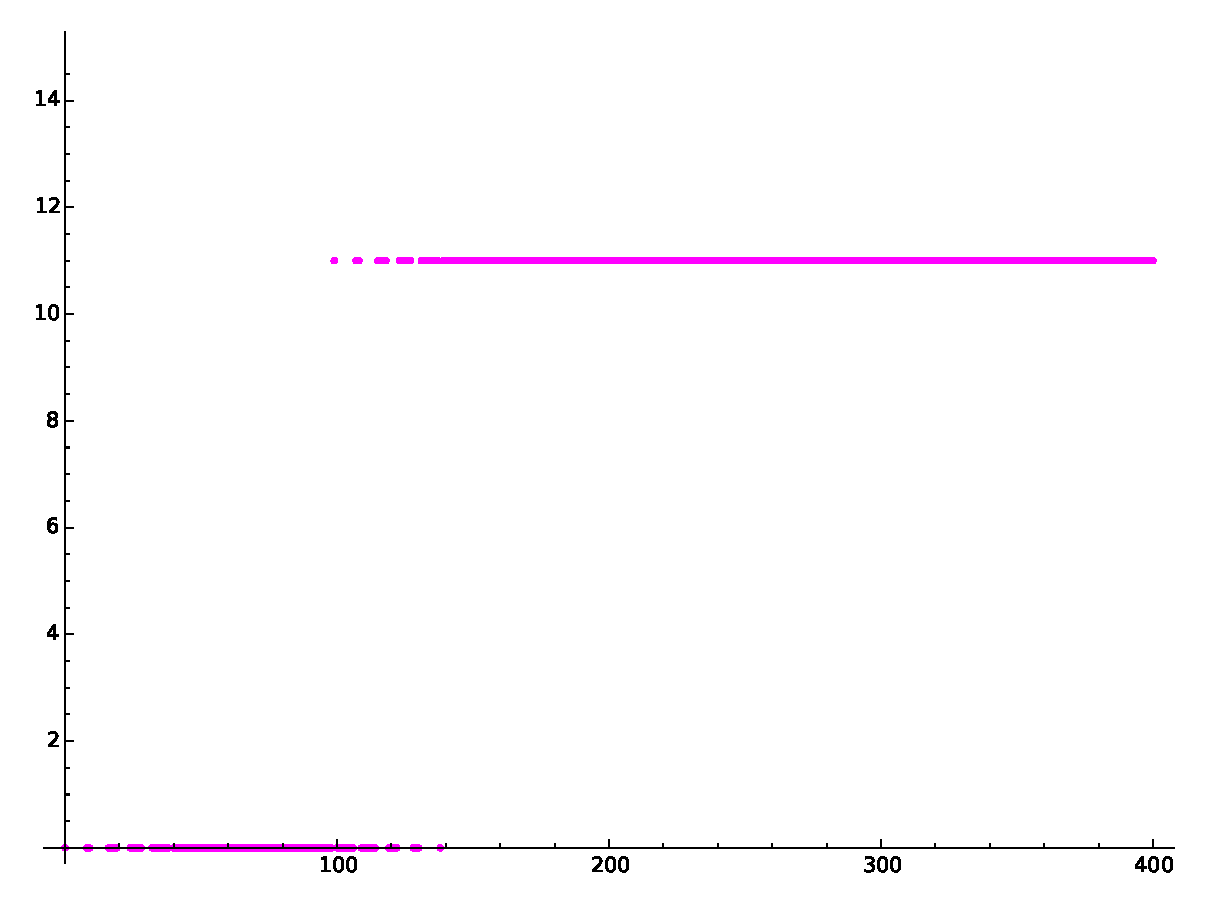
\includegraphics[scale=1.5]{equal.eps} \end{center}
%\end{block}


\begin{block}{When is $c_{mon}(M)>c(M)?$}
Given that the following two conditions hold, $c_{mon}(s)>c(s)$ for any element $s$ in any monoid $M$.
\begin{itemize}
\item $c_{eq}(s)>c_{adj}(s)$ 
\item If $s$ has two factorizations $z_1$ and $z_2$ of length $l$, there exists a factorization $z_3$ of length $q \neq l$ such that $d(z_1,z_3)<c_{eq}(s)$ and $d(z_2,z_3)<c_{eq}(s)$. 
\end{itemize}
\end{block}




\begin{block}{A Case Where $c_{mon}(M)>c(M)$}

Let $M=\langle na,na+n,2na+nx+1 \rangle$ with $x \geq 2$. Then 

\hfill
\begin{itemize}
\item $c_{eq}(M)=na+nx+1$
\item $c_{adj}(M)<na+nx+1$
\item $c_{mon}(M)=na+nx+1$
\item $c_{mon}(M)>c(M)$
\end{itemize}
\begin{example}
Let $M=\langle 8,10,21 \rangle$, so $n=2$, $a=4$, and $x=2$. Then $c_{eq}(M)=c_{mon}(M)=13$, and $c(M)=5$. Then $c_{mon}(M)>c(M)$. 
\end{example}
\end{block}


\begin{block}{$c_{mon}(M)-c(M)$ can be Arbitrarily Large}
\begin{minipage}[t]{0.58\linewidth}
\begin{center}
Monotone and Regular Catenary Degrees of $\langle a,a+1,\mathcal{F}\langle a,a+1\rangle \rangle$ \end{center}
\begin{center} \includegraphics[width=30cm]{plot.eps} \end{center}
\end{minipage}
\begin{minipage}[t]{0.38\linewidth}
\begin{itemize}
\vspace{2in}
\item $c_{mon}(M)=a^2-2a-1$
\item $c(M)=2a-3$
\item $c_{mon}(M)-c(M)=a^2-4a-4$
\end{itemize}
\vspace{2in}
For large $a$, this difference can grow arbitrarily large. 
\end{minipage}
\end{block}


\begin{block}{Conclusions}
\begin{itemize}
	\item In some monoids, namely those generated by arithmetic sequences, $c_{mon}(M)=c(M)$. 
	\item In generalized arithmetic monoids, we can have either $c_{mon}(M)>c(M)$ or $c_{mon}(M)=c(M)$. 
	\item In general, we expect that $c_{mon}(M)>c(M)$. In fact, the difference between the two can grow arbitrarily large. 
	\end{itemize}
\end{block}

\begin{block}{Acknowledgments}
\begin{itemize}
\footnotesize{
\item We would like to thank... 
\item Dr. Brian Wissman and Dr. Bob Pelayo for overseeing our research
\item Dr. Chris O'Neill and Dr. Scott Chapman for providing our research question and continuing support throughout this process
\item Dr. Brian Loft, Dr. Rebecca Garcia, Dr. Luis Garcia, and PURE Math for hosting us
\item This work was conducted during the 2014 PURE Math REU which is supported by the National Science Foundation (NSF Proposals DMS-1045147 and DMS-1045082).}
\end{itemize}
\vspace{-1ex}
\end{block}

\begin{block}{References}
\begin{itemize}
\footnotesize{
	\item Bowles, Craig, Scott T. Chapman, Nathan Kaplan, and Daniel Reiser. "On Delta Sets Of Numerical Monoids." \textit{Journal of Algebra and Its Applications J. Algebra Appl.} \textbf{05} (2006), 695-718. \\

	\item S. T. Chapman, M. Corrales, A. Miller, C. Miller, and D. Patel. \textit{The Catenary Degrees of Elements in Numerical Monoids Generated by Arithmetic Sequences}. Journal of the Australian Mathematical Society, 2014. \\
	
	\item S. T. Chapman, P. A. Garc�a-S�nchez, and D. Llena. "The Catenary and Tame Degree of Numerical Monoids." \textit{Forum Mathematicum} \textbf{21} (2009). \\


	\item A. Geroldinger and P. Yuan, The Monotone Catenary Degree of Krull Monoids, \textit{Results in Mathematics} \textbf{63}(2013), 999-1031. \\
	
		\item M. Omidali. "The Catenary and Tame Degree of Numerical Monoids Generated by Generalized Arithmetic Sequences." \textit{Forum Mathematicum}. \textbf{24} (2012), 627-640.

	\item A. Philip, A characterization of arithmetical invariants by the monoid of relations II: The monotone catenary degree and applications to semigroup rings, \textit{Semigroup Forum} \textbf{81} (2010), 424-434. \\
	
	\item J. C. Rosales and P. A. Garc\'ia-S\'anchez, \textit{Finitely generated commutative monoids}, Nova Science Publishers, NewYork, 1999.

}
\end{itemize}	

\end{block}


%%%%%%%%%%%%%%%%%%%%%%%%%%%%%%%%%%%%%%%%%%%%%%%%%%%%%%%

\end{column}
\end{columns}
\end{frame}
\end{document}


%%%%%%%%%%%%%%%%%%%%%%%%%%%%%%%%%%%%%%%%%%%%%%%%%%%%%%%%%%%%%%%%%%%%%%%%%%%%%%%%%%%%%%%%%%%%%%%%%%%%
%%% Local Variables: 
%%% mode: latex
%%% TeX-PDF-mode: t
%%% End: 
